\chapter{Experimental part: Models and evaluation}
\label{chap:model}
In this chapter, we will experiment with the different classification models. We will consider Random Forest, SVM, Extreme Random Forest \cite{ExtRF} and Logistic regression for comparison. Also, we will analyze the feature importance for every event component with Random Forest. We will actively use great Python library scikit-learn (sklearn).\\

We conducted three experiments with different preferences and input features. The result of every experiment is a summary table with the following metrics: accuracy, precision, recall and $F_1$ score. In this chapter, we also will briefly remind the definition and intuitive meaning every metric.\\

\section{Feature importance}
To gather the feature importance for every component, we will use Random Forest classifier. It's implementation in sklearn automatically calculates the "Gini importance" or "mean decrease impurity" which is defined as the total decrease in node impurity, weighted by the probability of reaching that node and then averaged over all trees of the ensemble.\\

For every event component, we trained Random Forest classifier with one-vs-all strategy. That means that as positive examples we choose the records from a dataset associated with the target event component and as negative examples the rest of records. After we had trained the Random Forest (the number of trees is 1000), we took the feature importance from it. The detailed procedure of building the model will be discussed in the next section.\\

Remarkably that the \textbf{Top-5} features for every component totally makes sense:

\begin{itemize}
    \item \textbf{Event name}: font family, tag, block width, font size, the number of uppercase letters. Usually, the title of the event is bigger and probably has a tag <h1>. The name is rather short, and hence the block width is small. The font size is large and the number of uppercase letters often higher for attracting the user. To see the importance of features for a name component see figure \ref{fig:importanceName}. The rest of related pictures you will find in \nameref{appendix}.
    \item \textbf{Event date}: digits share, the number of digits, font family, tag, number of punctuation. It also logical since the date, of course, has more digits than other web elements. The number of punctuation is rather small because the text is usually short. See figure \ref{fig:importanceDate}.
    \item \textbf{Event location}: number of uppercase letters, tag, font family, the number of siblings, text length. See figure \ref{fig:importanceLocation}.
    \item \textbf{Event description}: block width, text length, font family, number of punctuation. The description, typically, is a wider block of text, that's why block width and text length are the most important features. The number of punctuation is also correlated with the text length and means significant. See figure \ref{fig:importanceDescription}.
\end{itemize}

\begin{figure}[h]
\begin{center}
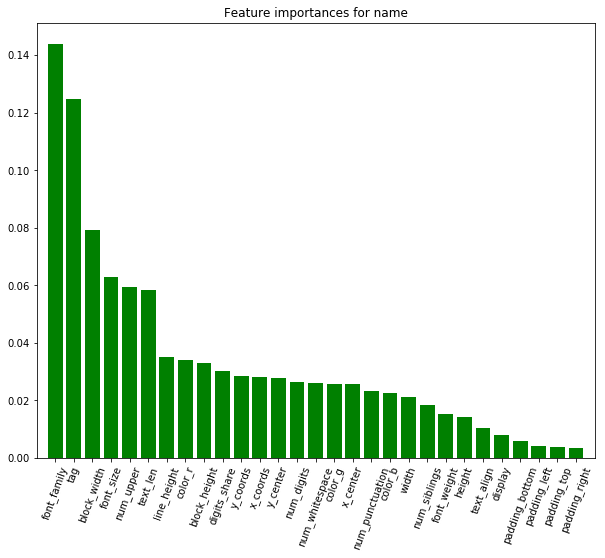
\includegraphics[width=1.0\textwidth]{figures08/importanceName}
\caption{Feature importance from Random Forest for the Event name. Top-5: font family, tag, block width, font size, number of uppercase letters}
\label{fig:importanceName}
\end{center}
\end{figure}


\section{Comparison of different models}

\subsection{Evaluation metrics}

We used standard metrics for binary classification problem and Information extraction task. All the values reach its best value at 1 and worst score at 0. See below brief description each of them.\\

\noindent\textbf{The mean accuracy} is the average number of incorrect predictions: 
$$ mean\_accuracy = \frac{tn + fp}{tp + tn + fp + fn}$$
where $tp$, $tn$, $fp$, $fn$ are accordingly true positives, true negatives, false positives and false negatives records from a predicted labels.\\

\noindent\textbf{The precision} is the ability of the classifier not to label as positive a sample that is negative:
$$precision = \frac{tp}{tp + fp}$$ \\

\noindent\textbf{The recall} is the ability of the classifier to find all the positive samples:
$$recall = \frac{tp}{tp + fn}$$ \\

\noindent\textbf{The $F_1$ score}, also known as balanced F-score or F-measure is as a weighted average of the precision and recall. The contribution of precision and recall to the $F_1$ score are equal. The formula for the $F_1$ is:
$$F_1 = 2 * \frac{precision * recall}{precision + recall}$$\\


\section{Experiments}

In this section, we will describe our experiments on building the binary classification models for every event component. For every test, we will change the preferences to see the difference and influence of each step.\\

For every binary classification model and target event component, we will do the following actions: 
\begin{enumerate}
    \item We select the \textit{target event component} for which we build the model (for example, date of the event)
    \item As positive examples, we take all records containing the target component in an original dataset ("startDate")
    \item As negative examples, we take the rest of the records
    and mark them as "no\_startDate" (records "name", "location", "description", "no\_event" will became "no\_startDate")
    \item We perform stratification procedure what means that we balance the dataset in such way that the number of examples for both classes would be the same.
    \item We impute missing values with the mean (we replaced outliers with NaN in the previous steps)
    \item We train the model
    \item We calculate four performance metrics like the average values after cross-validation procedure
    \item We build summary table and compare the results 
\end{enumerate}

For all experiments except the first one, we performed two additional procedures. Firstly, we do standardization of features with the mean and standard deviation. Secondly, we implemented custom cross-validation function which tracks the following important property: for every train-test split, domain names in both sets should not overlap. \\

The reason for performing this procedure is the following: we have many different URLs, but some of them come from the same domain name. Usually, the pages in one domain look similar, and it is not fair to train classifiers on certain pages and test on the pages from the same domain names. Our experimenting shows that if we don't do this procedure, the result of the classifier is overestimated. In our task and source code, we call this procedure \textit{fair train test split}.\\

\subsection{Experiment 1}
\noindent\textbf{Preferences:} Original numeric features as an input without tracking domain names intersection. \\

\noindent\textbf{Result:} All metrics value are very high, and the result is obviously overestimated. The reason for this is that both train and test dataset contained the same domain names. Therefore trained classifier has already known the design and properties of the website on the testing stage. See the table \ref{table:sumresultOriginal} to see extremely high metric values. The only SVM performs not well because it implies standardized values, but we didn't do it in the first experiment.\\

\noindent\textbf{Conclusion:} It is critical to keep training and testing examples independently and not allow to leak the information from the training stage to the testing stage. If you see the high values of performance metrics, be suspicious and try to understand why it happens.

\subsection{Experiment 2}
\noindent\textbf{Preferences:} Original numeric features with the tracking of domain names intersection while splitting into train and test subsets. \\

\noindent\textbf{Result:} After we added the restriction on domain names intersection, all the metrics decreased from .97 to .85 in average, but this estimation is much fair than previous. The result shows us that the model is working, but it's not the best, so we are motivated to tune it and experiment with the features further. Extreme Random Forest shows the best results for all event components. The event date component with SVM has the worst results by all metrics. Simple logistic regression shows the relatively good result for all models. See results of this experiment on the table \ref{table:sumresult}.\\     

\noindent\textbf{Conclusion:} Even if metrics decreased after applying some restrictions, it's better to have a fair model and optimize it.


\subsection{Experiment 3}
\noindent\textbf{Preferences:} Original numeric features with the tracking of domain names intersection while splitting into train and test subsets. Also, we extracted textual field and constructed a tf-idf \cite{tfidf} matrix which shows how important every word in a text relatively to the whole corpus. In our case, the corpus of documents is all textual fields from the dataset. We applied tf-idf transformation separately for train and test set. tf-idf matrix is sparse, that's why then we used Incremental PCA \cite{PCA} dimensionality reduction, which is more memory efficient than the traditional PCA. \\

\noindent\textbf{Result:} After these transformations the metric results for each event component and classifiers increased. Almost all metrics became greater than .8 for all components and classifiers. $F_1$ score, precision, and accuracy are the highest for Extreme Random Forest almost for all event components. The random forest has the highest recall for all components. See results of this experiment on the table \ref{table:sumresultPCA}.\\

\noindent\textbf{Conclusion:} Working with textual field and applying the combination of tf-idf and dimensional reduction methods can increase the result very much.\\

The code for all three experiments can be found on attached CD in the folder notebooks/ with the prefix \textit{"Model Building."}

% \subsection{Experiment 4}


\begin{table}[h]
\begin{center}
{\renewcommand{\arraystretch}{1.2}
\begin{tabular}{lrrrrll}
\toprule
f1\_score &  accuracy &  precision &  recall &    meta\_name &                  model \\
\midrule
\textbf{0.86} &           \textbf{0.86} &       \textbf{0.86} &    0.86 &         name &          Random forest \\
0.82 &           0.83 &       0.82 &    0.84 &         name &                    SVM \\
0.75 &           0.75 &       0.74 &    0.78 &         name &    Logistic regression \\
0.85 &           \textbf{0.86} &       0.81 &    \textbf{0.90} &         name &  Extreme Random Forest \\
\midrule
0.81 &           0.80 &       0.77 &    0.87 &     location &          Random forest \\
0.81 &           \textbf{0.81} &       \textbf{0.81} &    0.81 &     location &                    SVM \\
0.76 &           0.76 &       0.77 &    0.77 &     location &    Logistic regression \\
\textbf{0.82} &           \textbf{0.81} &       0.75 &    \textbf{0.91} &     location &  Extreme Random Forest \\
\midrule
0.84 &           0.83 &       0.82 &    0.88 &  description &          Random forest \\
0.82 &           0.82 &       0.78 &    0.87 &  description &                    SVM \\
0.77 &           0.77 &       0.74 &    0.83 &  description &    Logistic regression \\
\textbf{0.86} &           \textbf{0.87} &       \textbf{0.83} &    \textbf{0.91} &  description &  Extreme Random Forest \\
\midrule
\textbf{0.91} &           0.90 &       \textbf{0.90} &    0.92 &         date &          Random forest \\
0.87 &           0.87 &       0.89 &    0.86 &         date &                    SVM \\
0.80 &           0.81 &       0.86 &    0.79 &         date &    Logistic regression \\
\textbf{0.91} &           \textbf{0.91} &       0.88 &    \textbf{0.95} &         date &  Extreme Random Forest \\
\bottomrule
\end{tabular}}
\caption{Experiment 3: Metrics values for a different classification models and event components. PCA components calculated on extracted tf-idf matrix were added as additional features. Cross-validation with k = 5.}
\label{table:sumresultPCA}
\end{center}
\end{table} 

\section*{Conclusion of the chapter}

In this chapter we showed three experiment with four different classification models and initial preferences on input features. We saw that additionally constructed tf-idf matrix and PCA improved the performance, hence textual information is important factor for event extraction task. For every event component there are different classifiers which maximize the metrics, but generally ensemble model Extreme Random Forest works the best.